\section{Evaluation}

To evaluate our proposed architecture, two case studies of the prototype presented in Section \ref{PROTO} are presented. An Intel Core i7-4790K@3.60Ghz server with 8GB RAM DDR4 running Debian 8 was used. The prototype platform was configured to use L2 Sockets as the virtual network tool and NFs developed using both Python3 and/or CMR frameworks (depending on the performed test). All the experiments were repeated 30 times, considering a confidence level of 95\%.
% Each case study has its own metrics which must be considered to determine the feasibility of the architecture on the scenario.

%Our NFV environment consists of an emulated network topology running on two physical servers connected through a 1Gbps link. The first server has a  The other server is a Intel Core2Quad@2.66GHz, 4 Gigabytes of RAM and 500 Gigabytes of hard disk.
%The difference in resources of those two servers represents an heterogeneous environment where the developed platform must be able to function without any problems.
%By using OpenVSwitch and the KVM virtualization platform, emulated topologies consisting of connections between the VNF platform and virtual hosts can be deployed and modified in order to best represent the tested case study. In the next subsections the cases as well results from each of them are presented, with a subsection discussing the results of all cases.

\subsection{NSH for VNFs Intercommunication and SFC Steering}

In the first case study, we took advantage of the support for NSH to improve an existing NFV-based solution to mitigate DDoS attacks called DeMONS \cite{Garcia-2018}. In DeMONS, six separate VNFs were employed to detect malicious traffic and steer it through separate channels with different bandwidth capacities. These VNFs are Manager, Priority Classifier, Firewall, Allocator, Traffic Policing, and Router. The Manager is responsible for orchestrating the environment execution, for example, by monitoring the network load to scale running VNFs. The Priority Classifier, the Firewall, and the Allocator are responsible for identifying and classifying benign traffic, and blocking malicious traffic. Finally, both the Traffic Policing and the Router are responsible for applying user-defined policies (\textit{e.g.}, partial dropping and traffic shaping) on the suspicious flows.

% The first case study uses the prototype platform NSHP for coordinate the execution and communication between the VNFs which composes the DeMONS solution \cite{Garcia-2018}. The DeMONS is a NFV-based solution for Distributed Denial of Service (DDoS) attacks mitigation. Six different types of VNFs are employed in DeMONS architecture: Manager, Priority Classifier, Firewall, Allocator, Traffic Policing, and Routers. The Manager configures, starts and stops the other architecture elements. The Priority Classifier, the Firewall and the Allocator works together to identify and classify possible benign flows and block recognized malicious flows. Finally, the Traffic Policing and the Routers act on suspicious flows to apply restriction policies (\textit{e.g.}, partial dropping, traffic shaping) and create alternative routes.

In the original DeMONS solution, the first three VNFs (\textit{i.e.}, Priority Classifier, Firewall, and Allocator) are connected through a static path and share the traffic reputation through the Manager (acting as a central point of communication). The Priority Classifier uses Intrusion Detection System (IDS) techniques to generate the traffic reputation, and classifies the incoming flows with values ranging from 0 to 1. Reputation 0 means a malicious flow, reputation 1 indicates a benign flow, and values between those limits indicate unclassified traffic. After the classification, the traffic is forwarded to the Firewall, which queries the Manager to verify the traffic reputation, blocks 0 marked flows, and forwards the rest to the Allocator. The Allocator, in turn, steers the traffic to a high priority tunnel (that guarantees QoS for high reputation flows) or to a low priority tunnel (that can be overloaded with low reputation flows). Figure \ref{FIG:DeMONS}-A presents the original DeMONS implementation design.

% (\textit{i.e.}, level of confidence on the traffic classification)
% Our case study focuses on the relationship of the first three security VNFs (\textit{i.e.}, Priority Classifier, Firewall, and Allocator). In the DeMONS original solution, these elements are connected through a static path and communicate with each other beyond a shared reputation table located at the Manager VNF. The Priority Classifier applies Intrusion Detection System (IDS) techniques to the incoming flows and categorizes them by a floating value in the interval [0;1]. Reputation 0 indicates a malicious flow, while reputation 1 indicates a benign flow, values between them indicates the flow's suspecting level. This value is constantly updated and is saved in a table located in the Manager VNF. After the flow classification, the traffic is forwarded to the Firewall, this VNF queries the Manager table to check the incoming flows reputation and blocks 0 marked flows, forwarding the rest to the Allocator. The Allocator, in turn, steers the traffic to a high priority tunnel (that guarantee QoS for highest reputation flows) or to a low priority tunnel (for the lower reputation flows, this tunnel does not guarantee QoS and can operate overloaded). The Figure \ref{FIG:DeMONS}-A presents the original DeMONS implementation design.

\begin{figure}[!h]
\centering
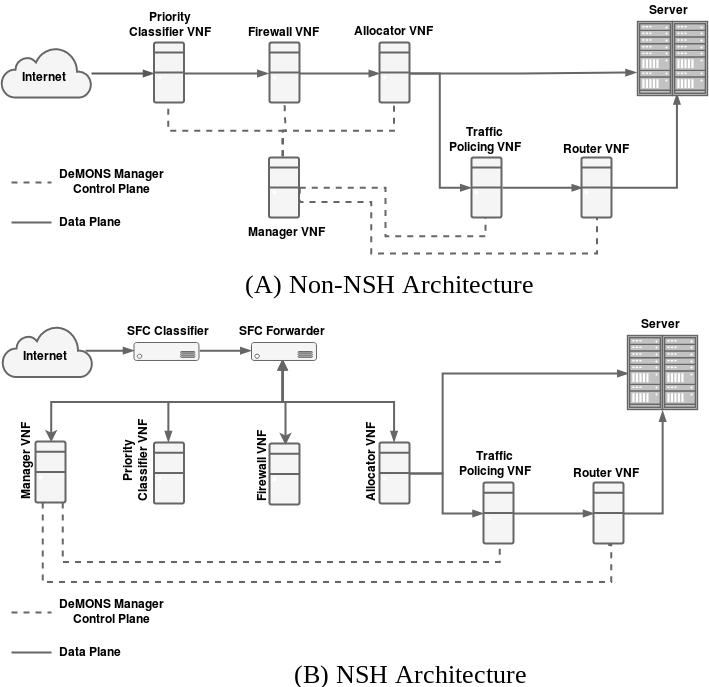
\includegraphics[width=.8\textwidth]{images/DeMONS.png}
\caption{DDoS Mitigation NFV Solution (DeMONS)}
\label{FIG:DeMONS}
\end{figure}


The DeMONS was deployed using the IETF's SFC architecture (\textit{i.e.}, Classifier and Service Function Forwarder) \cite{Joel-2015} and the VNF Platform prototype developed in this work. NSH was used to enable in-band control for sharing flow reputations and to orchestrate the traffic steering across all the employed NSH aware VNFs (\textit{i.e.}, the SFC). The reputation table (originally at the Manager) is now maintained by the Priority Classifier and shared between the VNFs through the NSH Context Header. In case of benign traffic, the Service Index is decremented by two in order to forward the packets directly to the Allocator, thus skipping the Firewall. Finally, the Allocator gets the reputation value directly from the flow packet by using the NSH's Context Header. Figure \ref{FIG:DeMONS}-B presents the adapted DeMONS implementation design.

% We deployed the DeMONS solution using the IETF's SFC architecture modules (\textit{i.e.}, Classifier and Service Function Forwarder) \cite{rfc7665} and the prototype VNF platform developed considering the architecture presented in Section \ref{ARCH}. We used the NSH to do in-band control of the flows reputations and coordination of the traffic steering across the DeMONS' SFC. We removed the shared reputation table from the Manager VNF and placed it locally at the Priority Classifier. The Priority Classifier uses that table and the IDS results to update the flow reputations, and, additionally, records the reputation value in the NSH's Context Header through the platform NSHP. Also, minor modifications were performed in the Priority Classifier NSHP's module in order to realized a double decremental in the Service Index for every flow with reputation greater than 0 during the NSH reinsertion. This Service Index manipulation skips the non-malicious traffic processing by the firewall, steering it directly to the Allocator. Finally, the Allocator gets the reputation value directly from the flow packet by using the NSHP's CH retrieve operation, without any VNF interaction. The Figure \ref{FIG:DeMONS}-B presents the adapted DeMONS implementation design.

The use of NSH led to performance improvements in DeMONS due to redesign and the embedded mechanism to exchange control data. The first experiment was executed to evaluate the execution time overhead introduced by retrieving and processing the reputations in both original and modified DeMONS. Two versions of the Packet Filter VNFC were developed in order to operate in both scenarios (NSH and Non-NSH), and were instrumented to measure the elapsed processing time for each packet. Iperf was used to generate the network traffic (UDP packets of 1470 Bytes), with the results presented in Figure \ref{FIG:DEMONSRRT}.

%Escala logaritimica
\begin{figure}[!htb]
\centering
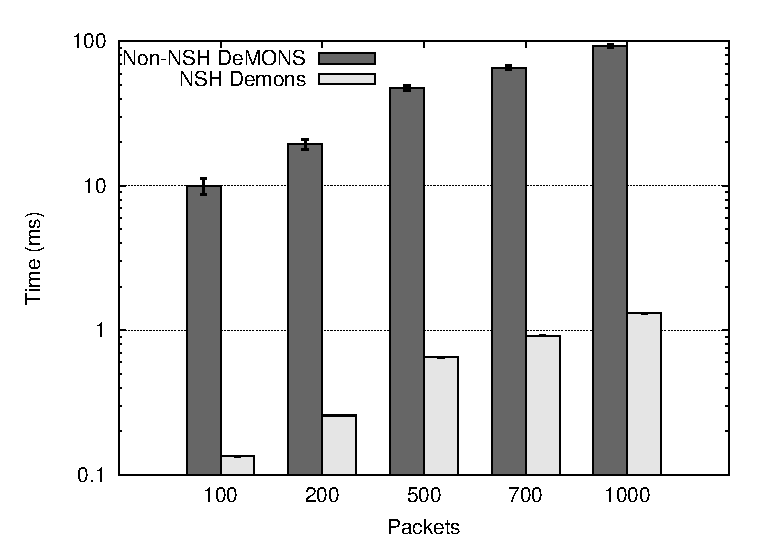
\includegraphics[width=.8\linewidth]{images/ExecTime.eps}
\caption{Reputation Retrieval Processing Time Overhead}
\label{FIG:DEMONSRRT}
\end{figure}

% \red{The use of NSH for the traffic steering and in-band control led to performance improvements in DeMONS. We analyzed the processing time overhead introduced by both the out band control (Non-NSH DeMONS) and in band control (NSH DeMONS) during the reputation retrieval for the DeMONS VNFs. To do that, an in band control VNFC and an out band control VNFC executing only the reputation retrieval operation were developed and deployed in the prototype platform. We instrumented the VNFCs in order to measure the execution time for every packet processed by them. Ours tests consists in traverse these VNFCs with 1470B UDP packets, created by the iperf tool, and aggregate the execution time for packets groups as exposed in Figure \ref{FIG:DEMONSRRT}.}

In the Non-NSH DeMONS, the reputation retrieval process consists in contacting the Manager (through a UDP Socket) to discover the reputations. This operation is performed for all the network packets traversing the VNFC. When NSH is employed, on the other hand, the reputation value is included in the NSH Context Header of each packet by the Priority Classifier. In this case, the Packet Filter just needs to open this header to retrieve the information. As suspected, the same operation (reputation retrieval) leads to significant differences in terms of processing time (in favor to NSH-based), which may affect other performance indicators (\textit{e.g.}, throughput and packet loss). An important observation is that no major differences occurred for packets with different sizes.
% \red{In the Non-NSH DeMONS, the reputation retrieval process consists on contacting the Manager (through an UDP Socket) to discover the reputations. This operation is performed for all the network packets traversing the VNFC. When NSH is employed, on the other hand, the reputation value is marked in the Context Header and its retrieving corresponds to just the local access of it. This operational difference leads to the Non-NSH DeMONS a reputation retrieval processing time overhead from 72 to 74 times greater than the NSH DeMONS. Once the extra processing time for this operation is imposed for each packet traversing the DeMONS VNFs, the RTT and throughput are directly affected according to the traffic volume growth. Also, it is important to notice that the package size do not change the reputation retrieval processing time (since the same operation is applied independently of this packet characteristic).}

The use of a Service Function Forwarder in the NSH DeMONS scenario also demonstrated interesting opportunities for improving the traffic steering overall. This SFC element (\textit{e.g.}, an OpenFlow Switch or a P4-enabled device) steers the network traffic according to the Service Index value present in the NSH Service Path Header. In this way, it is possible to manipulate the VNF execution order by updating the NSH Service Index according to decisions taken during VNF processing. For our case study, the Firewall VNF only processes the malicious traffic in order to collect statistics (\textit{e.g.}, number of discarded packets) and then discards the packets. In addition to not processing benign flows -- when malicious traffic is nonexistent (\textit{i.e.}, no attack occurring) -- it is possible to temporarily disable the Firewall VNF, thus saving computational resources.
% \red{Further, the traffic steering for the NSH DeMONS is more flexible than Non-NSH DeMONS due the use of a Service Function Forwarder. This SFC component steers the network traffic according to the Service Index present in the NSH Service Path Header. In this way, it is possible to manipulate the packet processing path by updating this NSH field according to decisions took during the VNFs processing. For our case study, the Firewall VNF only process the malicious traffic in order to collect statistics, such as the number of discarded packets, and finally drop it. In addition to not processing benign flows, when malicious traffic is inexistent (\textit{i.e.}, no attack occurring), its is possible to keep the Firewall VNF suspended, thus saving computational resources.}

%In Figure \ref{FIG:DEMONSFW}, for example, shows the aggregated processing time overhead measured internally for the Reputation Retrieval DeMONS VNFC (\textit{i.e.}, white box test), deployed in the prototype platform. Two different VNFCs were employed in this test: with out band control (Non-NSH DeMONS) and with in band control (NSH DeMONS). In the Non-NSH DeMONS, this processing consists on contacting the Manager (through an UDP Socket) to discover the reputations. This operation is performed for all the network packets traversing the network. When NSH is employed, on the other hand, the reputation value is marked in the Context Header and its retrieving corresponds to just the packet local access of it.

% and decide if the packet should be discarded (reputation equals to 0) or not.

% \blue{The application of NSH for the traffic steering and in band control makes possible to significantly improve the DeMONS NFs performance. For example, the Figure \ref{FIG:DEMONSFW} shows the aggregated packet processing time for the Firewall VNF with and without the use of NSH (developed using Python3 framework). The processing time measurement starts after the packet receiving by the NF, and stops before the packet sending operation. Thus, the Non-NSH DeMONS Firewall processing consists on the requisition of reputation value to the Manager (through a L3 UDP Socket) and the evaluation of that value in order to drop the packet (if it is 0) or forward it (other case). The NSH DeMONS Firewall, in turn, receives only the malicious traffic and a single operations is measured (\textit{i.e.}, the packet discarding). This operational difference between the Non-NSH DeMONS and NSH DeMONS Firewalls results in a large contrast in the processing time, being the first 72 to 77 times faster than the latter.}

%\red{In addition to the white box test, we analyzed the RTT overhead as a black box test for the same VNFCs also deployed in the prototype platform. To do that, we traversed the VNFs with an 1MBs UDP flow. The results seen in Figure \ref{FIG:DEMONSALLOC} show that the extra processing time introduced by the external reputation retrieval by the Non-NSH DeMONS is able to modify the average overall RTT when compared to the NSH DeMONS (difference of 0.2 milliseconds). Once the extra processing time for the reputation retrieval is imposed for every packet traversing the DeMONS VNFs, the RTT overhead may also grow for a higher traffic volume.}

%(also developed using Python3 framework) in order to measure the processing delay introduced by the reputation value retrieval

%\begin{figure}
%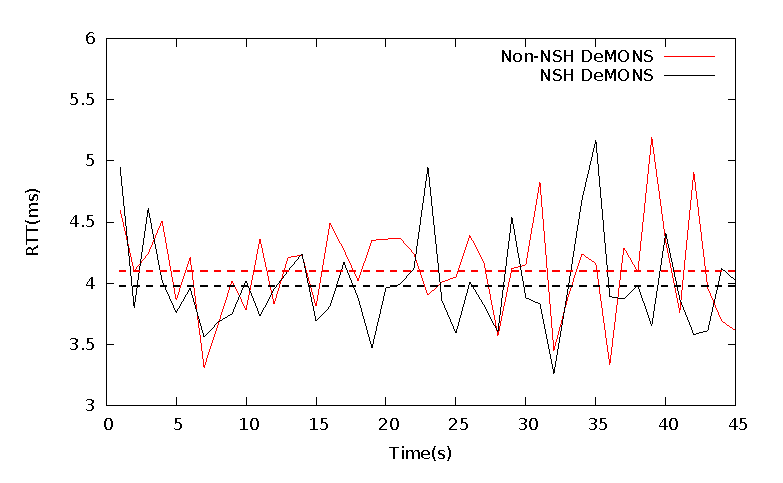
\includegraphics[width=\linewidth]{images/NSHAlloc.eps}
%\caption{Reputation Retrieval RTT}
%\label{FIG:DEMONSALLOC}
%\end{figure}

%%%%%
%\subsection{Heterogeneous Components Deployment}

%For the second case study, presented in Figure \ref{FIG:L7F}, the creation of a L7 Firewall employing the VNFC concept was evaluated. The ultimate goal of this network function is to block Skype traffic by using the fingerprint-based approach presented in \cite{Ehlert-2006}. The detection process consists on (i) port detection (80 and 443), (ii) payload pattern inspection (first 72 payload bytes), and (iii) the identification of similar data in different positions of the payload.

% In this case study we use the prototype platforms VNFCs support to deploy a complex function to realizing L7 filtering. We employed fingerprints presented in \cite{Ehlert-2006} to detect probable Skype traffic and block it. These fingerprints which are employed in this case study consists of port detection (80 and 443), payload pattern for port 443 (first 72 bytes), and payload segments self comparison for port 80.

%\begin{figure}[htb]
%\centering
%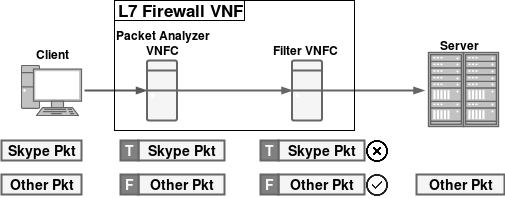
\includegraphics[width=.49\textwidth]{images/FirewallL7.png}
%\caption{L7 Firewall}
%\label{FIG:L7F}
%\end{figure}


%Two separate components were created: a packet analyzer and a packet filter. The packet analyzer was developed using the Python3 library Scapy\footnote{https://scapy.net/}, while the packet filter was implemented using both Python3 and CMR. The packet analyzer receives network traffic and verifies the destination port. All packets coming from ports 80/443 are marked and then forwarded, while the remaining packets are forwarded without marking. The marked packets received by the firewall are then processed in order to identify Skype fingerprints in the payload. If a Skype fingerprint is detected, the packet is marked as possible Skype. The second component (\textit{i.e.}, the packet filter) checks the marks and discards all the traffic that it considers to possibly be Skype traffic. These components were chained to create a L7 Firewall, although, they are independent and can be executed alone or be incorporated as part of other complex network functions.

% It is important to notice that the filter may block not only Skype traffic once, eventually, these Skype fingerprints can be employed by other applications.
% We developed a two components NF: Deep Packet Inspection (DPI) and a Firewall. The DPI was developed using Pyrhon3 language and Scapy library \footnote{https://scapy.net/}. This component receives the traffic and verifies the destination port. Every packet not addressed for port 80 or 443 is marked as non-Skype in the xxx byte of IP header and forwarded. The packets/frames addressed for port 80 and 443 are processed in order to identify the Skype fingerprints in the payload. After the payload analysis, if the processing returns true, the packet/frame is marked as possible Skype, else it is also marked as non-Skype. The second component (\textit{i.e.}, Firewall) checks the DPI marking and drops all the possible Skype traffic. It is important to notice that the Firewall may block not only SKype traffic once, eventually, these Skype fingerprints can be employed by other applications.

% We chained two components to create a sophisticated L7 Filter. These components, however, can be independently used or be incorporated as part of other complex functions. Also, we tested two firewalls implementations (\textit{i.e.}, Python3 and CMR) doing the same processing in order to identify performance differences between technologies combination. The case study is depicted in Figure \ref{FIG:L7F}.

%\begin{figure}[ht]
%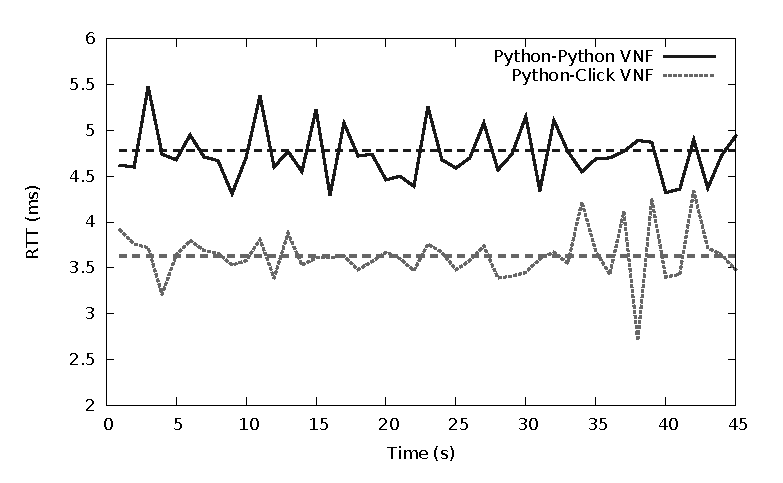
\includegraphics[width=\linewidth]{images/Delay.eps}
%\caption{L7 Firewall RTT}
%\label{FIG:L7FRTT}
%\end{figure}

% \vspace*{-1em}

%In this case study, we evaluated the RTT between the client and the server by using two combinations of VNFCS: both components were implemented in Python, and a mix of Python (for the Packet Analyzer) and CMR (for the Packet Filter). Figure \ref{FIG:L7FRTT} presents the results obtained from the experiments. It is possible to conclude that a combination of both programming languages is more appropriate to achieve better performance. It is important to notice, however, that although components implemented in CMR leverage its optimized packet processing, more sophisticated operations (\textit{e.g.}, analyzing the payload of ciphered packets) cannot be created using the default elements of this language. In these cases, Python 3 presents itself as an interesting approach to enable the development of advanced VNFCs with lower implementation efforts. Similar conclusions can be observed in other development scenarios, for example, when embedding assembly code in higher-level languages (\textit{e.g.}, C, C++), or when using the Java Native Interface (JNI) framework.
% \blue{Figure \ref{FIG:L7FRTT} presents the RTT measured during 45 seconds using Ping tool. Two VNFC combinations are employed in this test: the Python Packet Analyzer plus a Python Firewall, and the Python Packet Analyzer plus a CMR Firewall. The measured RTT varies from 4.4 to 5.5 milliseconds for python VNFCs combination, and from 2.9 to 4.4 for python and CMR combination. Once the same Python Packet Analyzer is used in both tests, the reduced RTT measurements verified by using a CMR Filter is attributed to its fastest modules, specially prepared for network traffic processing and previously compiled in a low-level programming language (C++). Despite presenting worse results in the RTT test, the Python3 programming framework still being an important piece to achieving higher flexibility and agility during the NFs development. Because of its general purpose, Python3 enables the implementation of sophisticated VNFCs (\textit{e.g.}, the presented Packet Analyzer) with lower efforts when compared to closed and monolithic frameworks, such as CMR.}
